\documentclass[11pt,table]{article}
% DEFINE COMMANDS

\usepackage{NotesTeX}

\usepackage[font=small,labelfont=bf]{caption}
\usepackage{enumerate}
\usepackage{amsmath,amssymb,amscd,amsfonts}
\usepackage{xcolor}
\usepackage{color}

\usepackage{tikz}
\usepackage{tikz-cd}
\tikzcdset{every label/.append style = {font = \small}}
\tikzcdset{row sep/normal=3.5em}
\tikzcdset{column sep/normal=3.5em}

\usetikzlibrary{matrix}
\usetikzlibrary{decorations.markings,calc,shapes}
\usetikzlibrary{positioning}
\usepackage{graphicx}
\usepackage{empheq}
\usepackage{physics}
\usepackage{siunitx}
\usepackage{tensor}

\usepackage{multicol}

\usepackage{youngtab}
\usepackage{cancel}
\usepackage{caption}
\usepackage{graphicx}
\usepackage{subcaption}
\usepackage{hyperref}



\title{{\Huge General Relativity}\\{\Large{Class 27}}} %replace with class number
\author{F. Spencer Stubbs}

\emailAdd{recnepsknarf@gmail.com} %replace with your email
\begin{document}
    \maketitle
    \flushbottom
    \newpage
    \pagestyle{fancynotes}
    \part{Birkhoff's Theorem and\\ Time Symmetry}
    
        \section{Spherically symmetric spacetime}\label{sec:intro}
            So far we have focused on spherically symmetric spacetimes which have three killing vector fields, namely in the directions of the three possible rotations of a sphere.  This gave us a very general metric of the form:
            \begin{align}\label{eq:GenMet}
                ds^2 = -e^{2\alpha (t,r)}dt^2 + e^{2\beta (t,r)}dr^2 + r^2d\Omega^2.
            \end{align}
            This metric can be applied to any spherically symmetric spacetime; physically this could be a spherically symmetric matter distribution with stress-energy $\tensor{T}{_\mu_\nu}$, or the vacuum around such a body where the stress-energy tensor is 0.  Since the general spherically symmetric metric is in principle time dependent, this can also describe time dependent processes which maintain spherical symmetry such as stellar collapse or expansion.
            
            Presently we will be interested in spherically symmetric vacuum solutions to the Einstein Field Equations:
            \begin{align}\label{eq:VacEqn}
                R_{\mu\nu} - \frac{1}{2}Rg_{\mu\nu} = 0
            \end{align}
            where $g_{\mu\nu}$ has the form \eqref{eq:GenMet} and see what further restrictions this has on the metric.
            
        \section{Birkhoff's Theorem}\label{sec:bkhfsthm}
            We know that that the condition $T_{\mu\nu}=0$ implies $R=0$ from the trace of the Einstein Field Equations (EFE), We can then plug this into the vacuum EFE to get that $R_{\mu\nu}=0$ must also be true.  We can use this to put further restrictions on our general metric \eqref{eq:GenMet}.  Doing some of the calculations we find:
            \begin{align}
                &R_{tr}=\frac{2}{r}\partial_t\beta(t,r) = 0\label{eq:Rtr}\\
                &R_{\theta\theta}=R_{\phi\phi}=e^{-2\beta(t,r)}[r(\partial_r\beta(t,r)-\partial_r\alpha(t,r))-1]+1 = 0\label{eq:Rpp}
            \end{align}
            The first of these tells us that $\beta(t,r)$ is in fact only a function of $r$, $\beta(r)$.  We can use this fact and apply $\partial_t$ to the second of these equations to obtain
            \begin{align*}
                \partial_t R_{\theta\theta} = e^{-2\beta(r)}(-r\partial_t\partial_r\alpha(t,r))=0
            \end{align*}
            Now this doesn't force $\alpha(t,r)$ to be solely a function of $r$, but it does allow us to write $\alpha$
            \begin{align}
                \alpha(t,r)&= f(r)+h(t)\\
                \implies g_{tt}dt^2&=-e^{2f(r)}e^{2h(t)}dt^2\label{eq:alpharestriction1}
            \end{align}
            We have used a lot of out coordinate freedom to simplify the metric to this point, but we still have some room.  Since $t$ is an arbitrary time coordinate we can always reparameterize it to some $t'(t)$.
            \sn{We can't do this with r due to the status we have given r as an "areal radius"} With this freedom we will choose $t'$ such that
            \begin{align}
                (dt)^2=e^{-2h(t)}(dt')^2.
            \end{align}
            (Note that we can still add in a constant term to this parameterization without ruining our time-independence, a fact which will be used later).  Now, after all of this our metric has the form
            \begin{align}\label{GenMet2}
                ds^2 = -e^{2\alpha(r)}dt^2+e^{2\beta(r)}dr^2 +
                r^2d\Omega^2,
            \end{align}
            which is completely time independent!\sn{Note that we have relabeled $f(r)=\alpha(r)$ and $t'=t$ out of convenience}  The manifest time independence of \eqref{GenMet2} tells us there exists a killing vector field $\Vec{K}$ such that
            $$
            \Vec{K} = \vec{\partial_t}.
            $$
            The existence of this killing vector field for this spacetime is known as Birkhoff's theorem which is stated as:
            \begin{quote}
                \it{The unique vacuum spherically symmetric spacetime is static.}
            \end{quote}
            Now, in the next section we will define what is meant by a "static spacetime" and in part II we will go on to show that this unique spherically symmetric vacuum solution is in fact the Schwarzschild spacetime.
            
        \section{Time Symmetry}\label{sec:TimeSym}
            \begin{itemize}
                \item A $stationary\ spacetime$ has a killing vector field which is timelike near spatial infinity.
                \sn{Stationary does not mean standing still.}
                \sn{The killing vector field does not need to be timelike everywhere, note that in the Schwarzschild spacetime $\Vec{K} = \vec{\partial_t}$ which implies $K^{\mu}K_{\mu}=g_{tt}=-(1-\frac{2M}{r})$ which is timelike for large r, but becomes spacelike inside of the event horizon.}
                
                \item A $static\ spacetime$ is stationary and time-reversal symmetric.  This causes the killing vector field to be normal to a set of $t=const.$ hypersurfaces.
            \end{itemize}
    
            We now want to take a moment to expand on this hypersurface point made in the above definition of a static spacetime.  Remember that not every 1-form is the gradient of a function, those that do satisfy $\omega = df$ are known as $exact$.  We can have a variety of other 1-forms, but an obvious non-exact choice would be 
            $$
            \omega = h(x^{\mu})df
            $$
            where $h(x^{\mu})$ is an arbitrary scalar function on our manifold.  These are known as "Twist-free" 1-forms and they are normal to hypersurfaces in the manifold, specifically, if $\omega_{\mu} = h(x^{\nu})\partial_{\mu}f$ then $\omega^{\mu}$ is normal to the $f=const.$ hypersurfaces.
            \sn{We can check if a one form is twist-free by checking if its components satisfy $\omega_{[\mu}\nabla_{\nu}\omega_{\rho]}=0$}
    
            There is a way to visualize what these different 1-forms mean.  As we discussed in a previous lecture, we can think of 1-forms as a bunch of planes in space.  when we place a vector in that space, the number of planes it pierces tells us information about the 1-forms action on that vector.  In the case where the 1-form is exact, these planes are parallel
            \vspace{.25in}
            \begin{center}    
            

\tikzset{every picture/.style={line width=0.75pt}} %set default line width to 0.75pt        

\begin{tikzpicture}[x=0.75pt,y=0.75pt,yscale=-1,xscale=1]
%uncomment if require: \path (0,300); %set diagram left start at 0, and has height of 300

%Shape: Rectangle [id:dp5110012504864849] 
\draw   (346.63,73.67) -- (399.5,85.1) -- (262.37,94.33) -- (209.5,82.9) -- cycle ;
%Shape: Rectangle [id:dp8090368899919016] 
\draw   (347.63,98.67) -- (400.5,110.1) -- (263.37,119.33) -- (210.5,107.9) -- cycle ;
%Shape: Rectangle [id:dp05120717442319145] 
\draw   (344.63,119.67) -- (397.5,131.1) -- (260.37,140.33) -- (207.5,128.9) -- cycle ;
%Straight Lines [id:da44132684458737925] 
\draw    (286.5,139) -- (273.5,157) ;
%Straight Lines [id:da46675174694338195] 
\draw    (300.5,117) -- (290.5,132) ;
%Straight Lines [id:da7732868120025449] 
\draw    (317.5,91) -- (305.5,109) ;
%Straight Lines [id:da7775072079648131] 
\draw    (333.84,65.5) -- (323.5,81) ;
\draw [shift={(335.5,63)}, rotate = 123.69] [fill={rgb, 255:red, 0; green, 0; blue, 0 }  ][line width=0.08]  [draw opacity=0] (8.93,-4.29) -- (0,0) -- (8.93,4.29) -- cycle    ;




\end{tikzpicture}
            \end{center}

            However, if the 1-form is twist-free the angle between these planes smoothly varies due to the function $h(x^{\mu})$'s influence
            \vspace{.25in}
            \begin{center}
    

            \tikzset{every picture/.style={line width=0.75pt}} %set default line width to 0.75pt        

            \begin{tikzpicture}[x=0.75pt,y=0.75pt,yscale=-1,xscale=1]
%uncomment if require: \path (0,300); %set diagram left start at 0, and has height of 300

%Shape: Rectangle [id:dp4094217360003136] 
\draw   (387.51,38.53) -- (252.69,67.08) -- (183.49,69.47) -- (318.31,40.92) -- cycle ;
%Shape: Rectangle [id:dp6677998764378119] 
\draw   (390.5,102) -- (252.69,102) -- (184.5,90) -- (322.31,90) -- cycle ;
%Shape: Rectangle [id:dp10371544585166825] 
\draw   (384.83,150.47) -- (248.61,129.62) -- (183.02,107.44) -- (319.24,128.29) -- cycle ;
%Straight Lines [id:da03748611254451939] 
\draw    (272.5,133) -- (266.5,143) ;
%Straight Lines [id:da4931789518481051] 
\draw    (289.5,102) -- (275.5,127) ;
%Straight Lines [id:da9060549780491587] 
\draw    (300.5,83) -- (293.5,96) ;
%Straight Lines [id:da749778393168705] 
\draw    (306.08,72.64) -- (300.5,83) ;
\draw [shift={(307.5,70)}, rotate = 118.3] [fill={rgb, 255:red, 0; green, 0; blue, 0 }  ][line width=0.08]  [draw opacity=0] (8.93,-4.29) -- (0,0) -- (8.93,4.29) -- cycle    ;




\end{tikzpicture}
            \end{center}

            Meanwhile, there are plenty of 1-forms which satisfy neither of these conditions, and these usually don't have planes that "knit together" over the whole spacetime. For example, they may abruptly change direction
            \vspace{.25in}
            \begin{center}
    



            \tikzset{every picture/.style={line width=0.75pt}} %set default line width to 0.75pt        

            \begin{tikzpicture}[x=0.75pt,y=0.75pt,yscale=-1,xscale=1]
%uncomment if require: \path (0,352); %set diagram left start at 0, and has height of 352

%Shape: Rectangle [id:dp4094217360003136] 
\draw   (372.91,55.56) -- (235.38,46.77) -- (168.09,30.44) -- (305.62,39.23) -- cycle ;
%Shape: Rectangle [id:dp6677998764378119] 
\draw   (375.5,91) -- (237.69,91) -- (169.5,79) -- (307.31,79) -- cycle ;
%Shape: Rectangle [id:dp10371544585166825] 
\draw   (371.94,112.2) -- (235.03,127.87) -- (165.91,123.71) -- (302.82,108.03) -- cycle ;
%Shape: Rectangle [id:dp959972474963547] 
\draw   (416.23,182.88) -- (396.69,37.05) -- (398.5,-7) -- (418.04,138.84) -- cycle ;
%Shape: Rectangle [id:dp7038320466014627] 
\draw   (446.23,195.52) -- (426.69,49.68) -- (428.5,5.63) -- (448.04,151.47) -- cycle ;
%Shape: Rectangle [id:dp9428961346863489] 
\draw   (473.23,204.88) -- (453.69,59.05) -- (455.5,15) -- (475.04,160.84) -- cycle ;




\end{tikzpicture}
            \end{center}
            Bringing this all together: we can have timelike killing vector fields which are not hypersurface-orthogonal, these simply define stationary spacetimes.  But, if the spacetime is static, we can envision it as a foliation of spacelike hypersurfaces which are orthogonal to the timelike killing vector field.

            So, how does all of this help us?  Well here is a practical perspective.  If we use $t$ as our time coordinate so that $\Vec{K} = \vec{\partial_t}$, then out stationary spacetime can have timelike cross terms and our static one cannot:

            \begin{equation}
                ds^2=g_{00}dt^2 + g_{0i}(dtdx^i+dx^idt)+g_{ij}dx^idx^j\tag{stationary}
            \end{equation}
            \begin{equation}
                ds^2=g_{00}dt^2 +g_{ij}dx^idx^j\tag{static}
            \end{equation}
            \vspace{.25in}

            Where $g_{\mu\nu}$ is time-independent.  An example of this is a rotating black hole.  The Kerr metric has cross terms as displayed above, and there is clearly no time-reversal symmetry because if you change the flow of time the rotation changes direction, thus the Kerr spacetime is stationary.  

\newpage
    \part{Deriving Schwarzschild}
        \section{The unique spherically symmetric vacuum solution}
            We want to take our metric \eqref{GenMet2} and use the freedom left from $R_{\mu\nu}=0$ to apply more restrictions to it.  Using the remaining terms we know that 
            \begin{align*}
                e^{\beta(r)-\alpha(r)}R_{tt}+R_{rr}=\frac{2}{r}(\partial_r\alpha(r)+\partial_r\beta(r))=0\\
                \implies\partial_r(\alpha(r)+\beta(r))=0\\
            \end{align*}
            Integrating we get
            \begin{align}
                \alpha(r)=-\beta(r) + C
            \end{align}
            Which gives us a term in the line element of the form
            \begin{align*}
                e^{2\alpha(r)}dt^2 = e^{-2\beta(r)}e^{2C}dt^2
            \end{align*}
            Using the fact we mentioned before about being able to reparameterize up to a constant in the time coordinate we can remove this extra term by defining $t'$ such that
            \begin{align*}
                dt^2=e^{-2C}(dt')^2.
            \end{align*}
            Which essentially sets $C=0$ and thus gives us
            \begin{align}\label{eq:alphbet}
                \alpha(r)=-\beta(r).
            \end{align}
            So, we have managed to recast the entire metric in terms of a single function $\alpha(r)$.  In doing this we have exhausted all of the useful components of $R_{\mu\nu}$ besides the angular terms $R_{\theta\theta}=R_{\phi\phi}$ (we previously used the time derivative of these terms, not the terms themselves).  Finally, using \eqref{eq:alphbet} we obtain
            \begin{align*}
                R_{\theta\theta}=e^{-2\beta(r)}[r(\partial_r\beta(r)-\partial_r\alpha(r))-1]+1 = 0\\
                \implies e^{2\alpha(r)}(2r\partial_r\alpha(r) +1)=1\\
                \implies r\partial_re^{2\alpha(r)}+e^{2\alpha(r)}\partial_rr=1\\
                \implies\partial_r(re^{2\alpha(r)}) = 1
            \end{align*}
            which we can integrate to obtain
            \begin{align}
                e^{2\alpha(r)}=1+\frac{C}{r}
            \end{align}
            comparing this metric to the weak field limit around a point mass (which we know must equal this metric by the uniqueness condition in Birkhoff's theorem), we can see that $C=2M$ and thus our spherically symmetric vacuum solution is 
            \begin{align}
                ds^2 = -\left(1-\frac{2M}{r}\right)dt^2+\frac{1}{1-\frac{2M}{r}}dr^2 + r^2d\Omega^2
            \end{align}
            the Schwarzschild metric!
            
            Take note that the fact the solution exists at all is very suprising because we usually cannot solve nonlinear PDE's exactly.  Futher the fact that this is a solution to a nonlinear PDE means that we can't simply add these solutions together to get, say, the metric around two black holes.  We can however invoke Birkhoff's theorem to state that since this solution is the unique spherically symmetric vacuum solution, any spherically symmetric matter distribution undergoing a spherically symmetric time-dependent process (such as stellar collapse) will have the vacuum around it be the Schwarzschild spacetime.  This necessarily implies that there are no spherical waves in General Relativity since the Schwarzschild metric is time-independent.
        \section{Curvature of the Schwarzschild spacetime}
            Now that we know about the Schwarzschild spacetime we can ask questions about the full Riemann tensor $\tensor{R}{^\mu_\nu_\rho_\sigma}$.  For instance: are the singularities at $r=2M$ and $r=0$ actual defects in the manifold or are they simply artifacts of poor chart choices? Unfortunately the Riemann tensor has a complicated coordinate dependence and in the Schwarzschild coordinates the answer is that $\tensor{R}{^\mu_\nu_\rho_\sigma}$ is singular at both of these points. However, scalar fields, unlike higher rank tensor fields, have a very simple coordinate dependence
            \begin{align*}
                \phi(x^{\mu})\rightarrow\phi(x^{\mu'})=\phi(x^{\mu}(x^{\mu'}))
            \end{align*}
            So we can look at the scalar field $R$ determined by the Ricci scalar to see if we can gain any knowledge about these singularities.  Well, if we calculate $R$
            \begin{align}
                R=\tensor{R}{^\mu^\nu^\rho^\sigma}\tensor{R}{_\mu_\nu_\rho_\sigma}=\frac{48M^2}{r^6}
            \end{align}
            we see that there is no curvature singularity at $r=2M$ but there is at $r=0$, implying that $r=2M$ is in fact a coordinate singularity while $r=0$ is a true singularity of the manifold. This means we can look at some of the experiences of observers as they pass from $r=2M$ to $r=0$.
            \begin{itemize}
                \item The first interesting result is that an observer travels from a point at $r>2M$ to $r=0$ in finite proper time on their worldline.  This is peculiar given that an observer at infinity will see the infalling observer stuck on the event horizon.
                \item The second interesting result is that the tidal forces felt by an extended object as they pass from $r=2M$ to $r=0$ compress the body along the direction perpendicular to their motion and stretch it along the direction parallel to their motion. This process, illustrated below has the very technical name "spaghettification"
                \begin{center}
                    

                

                \tikzset{every picture/.style={line width=0.75pt}} %set default line width to 0.75pt        

                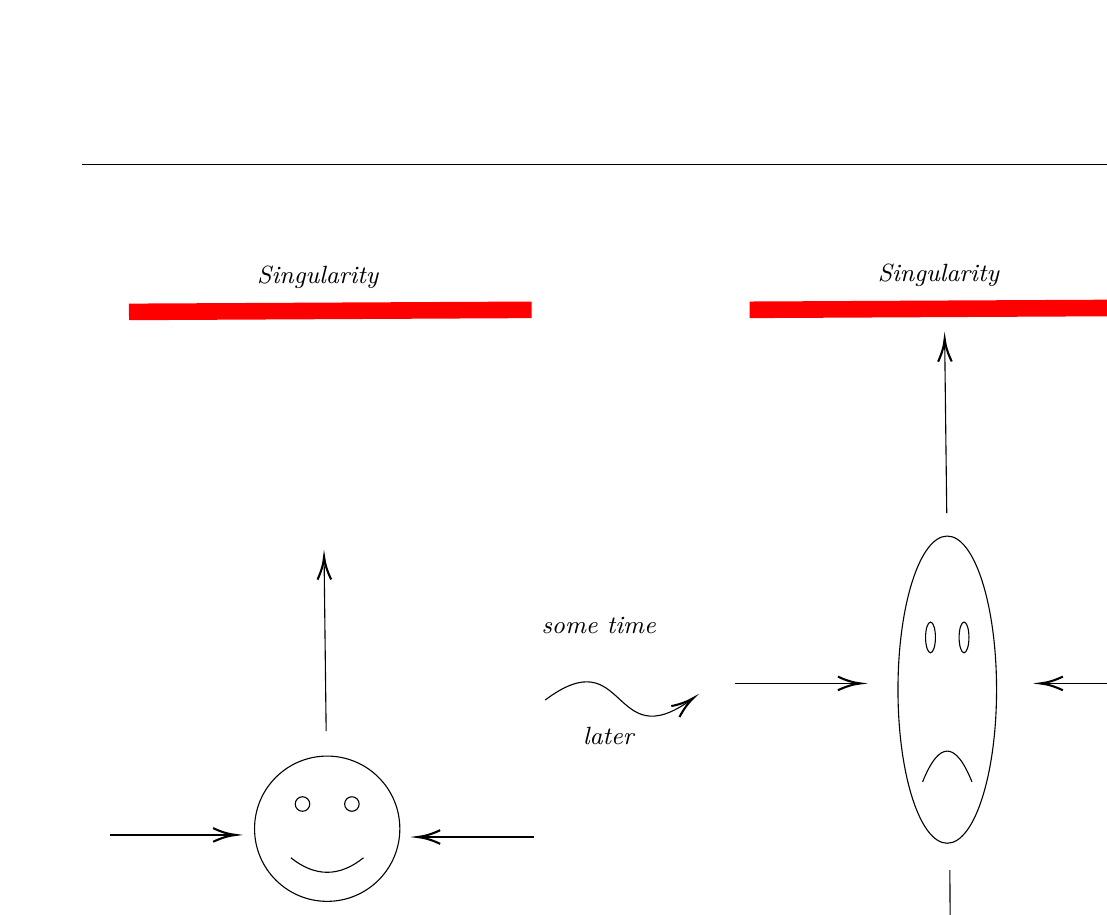
\begin{tikzpicture}[x=0.75pt,y=0.75pt,yscale=-1,xscale=1]
%uncomment if require: \path (0,424); %set diagram left start at 0, and has height of 424

%Shape: Smiley Face [id:dp8434513976943787] 
\draw   (107,281) .. controls (107,261.67) and (122.67,246) .. (142,246) .. controls (161.33,246) and (177,261.67) .. (177,281) .. controls (177,300.33) and (161.33,316) .. (142,316) .. controls (122.67,316) and (107,300.33) .. (107,281) -- cycle ; \draw   (126.6,269.1) .. controls (126.6,267.17) and (128.17,265.6) .. (130.1,265.6) .. controls (132.03,265.6) and (133.6,267.17) .. (133.6,269.1) .. controls (133.6,271.03) and (132.03,272.6) .. (130.1,272.6) .. controls (128.17,272.6) and (126.6,271.03) .. (126.6,269.1) -- cycle ; \draw   (150.4,269.1) .. controls (150.4,267.17) and (151.97,265.6) .. (153.9,265.6) .. controls (155.83,265.6) and (157.4,267.17) .. (157.4,269.1) .. controls (157.4,271.03) and (155.83,272.6) .. (153.9,272.6) .. controls (151.97,272.6) and (150.4,271.03) .. (150.4,269.1) -- cycle ; \draw   (124.5,295) .. controls (136.17,304.33) and (147.83,304.33) .. (159.5,295) ;
%Straight Lines [id:da13002839824666856] 
\draw    (37.5,284) -- (96,284) ;
\draw [shift={(98,284)}, rotate = 180] [color={rgb, 255:red, 0; green, 0; blue, 0 }  ][line width=0.75]    (10.93,-3.29) .. controls (6.95,-1.4) and (3.31,-0.3) .. (0,0) .. controls (3.31,0.3) and (6.95,1.4) .. (10.93,3.29)   ;
%Straight Lines [id:da6365727193590709] 
\draw    (241.5,285) -- (187.5,285) ;
\draw [shift={(185.5,285)}, rotate = 360] [color={rgb, 255:red, 0; green, 0; blue, 0 }  ][line width=0.75]    (10.93,-3.29) .. controls (6.95,-1.4) and (3.31,-0.3) .. (0,0) .. controls (3.31,0.3) and (6.95,1.4) .. (10.93,3.29)   ;
%Straight Lines [id:da7653309342738577] 
\draw    (141.5,234) -- (140.52,152) ;
\draw [shift={(140.5,150)}, rotate = 449.32] [color={rgb, 255:red, 0; green, 0; blue, 0 }  ][line width=0.75]    (10.93,-3.29) .. controls (6.95,-1.4) and (3.31,-0.3) .. (0,0) .. controls (3.31,0.3) and (6.95,1.4) .. (10.93,3.29)   ;
%Straight Lines [id:da9119877029723271] 
\draw    (141,333) -- (141.49,419) ;
\draw [shift={(141.5,421)}, rotate = 269.67] [color={rgb, 255:red, 0; green, 0; blue, 0 }  ][line width=0.75]    (10.93,-3.29) .. controls (6.95,-1.4) and (3.31,-0.3) .. (0,0) .. controls (3.31,0.3) and (6.95,1.4) .. (10.93,3.29)   ;
%Straight Lines [id:da07354860345266045] 
\draw [color={rgb, 255:red, 255; green, 0; blue, 0 }  ,draw opacity=1 ][line width=6]    (46.5,32) -- (240.5,31) ;
%Curve Lines [id:da2803430979774071] 
\draw    (247,219) .. controls (286.6,189.3) and (278.67,246.83) .. (317.31,218.87) ;
\draw [shift={(318.5,218)}, rotate = 503.13] [color={rgb, 255:red, 0; green, 0; blue, 0 }  ][line width=0.75]    (10.93,-3.29) .. controls (6.95,-1.4) and (3.31,-0.3) .. (0,0) .. controls (3.31,0.3) and (6.95,1.4) .. (10.93,3.29)   ;
%Shape: Smiley Face [id:dp790774689410644] 
\draw   (417,214) .. controls (417,173.13) and (427.63,140) .. (440.75,140) .. controls (453.87,140) and (464.5,173.13) .. (464.5,214) .. controls (464.5,254.87) and (453.87,288) .. (440.75,288) .. controls (427.63,288) and (417,254.87) .. (417,214) -- cycle ; \draw   (430.3,188.84) .. controls (430.3,184.75) and (431.36,181.44) .. (432.68,181.44) .. controls (433.99,181.44) and (435.05,184.75) .. (435.05,188.84) .. controls (435.05,192.93) and (433.99,196.24) .. (432.68,196.24) .. controls (431.36,196.24) and (430.3,192.93) .. (430.3,188.84) -- cycle ; \draw   (446.45,188.84) .. controls (446.45,184.75) and (447.51,181.44) .. (448.83,181.44) .. controls (450.14,181.44) and (451.2,184.75) .. (451.2,188.84) .. controls (451.2,192.93) and (450.14,196.24) .. (448.83,196.24) .. controls (447.51,196.24) and (446.45,192.93) .. (446.45,188.84) -- cycle ; \draw   (428.88,258.4) .. controls (436.79,238.67) and (444.71,238.67) .. (452.63,258.4) ;
%Straight Lines [id:da6930483662776623] 
\draw    (338.5,211) -- (397,211) ;
\draw [shift={(399,211)}, rotate = 180] [color={rgb, 255:red, 0; green, 0; blue, 0 }  ][line width=0.75]    (10.93,-3.29) .. controls (6.95,-1.4) and (3.31,-0.3) .. (0,0) .. controls (3.31,0.3) and (6.95,1.4) .. (10.93,3.29)   ;
%Straight Lines [id:da8264574597290069] 
\draw    (541.5,211) -- (487.5,211) ;
\draw [shift={(485.5,211)}, rotate = 360] [color={rgb, 255:red, 0; green, 0; blue, 0 }  ][line width=0.75]    (10.93,-3.29) .. controls (6.95,-1.4) and (3.31,-0.3) .. (0,0) .. controls (3.31,0.3) and (6.95,1.4) .. (10.93,3.29)   ;
%Straight Lines [id:da0818458153130508] 
\draw    (440.5,129) -- (439.52,47) ;
\draw [shift={(439.5,45)}, rotate = 449.32] [color={rgb, 255:red, 0; green, 0; blue, 0 }  ][line width=0.75]    (10.93,-3.29) .. controls (6.95,-1.4) and (3.31,-0.3) .. (0,0) .. controls (3.31,0.3) and (6.95,1.4) .. (10.93,3.29)   ;
%Straight Lines [id:da7282155142408508] 
\draw    (442,301) -- (442.49,387) ;
\draw [shift={(442.5,389)}, rotate = 269.67] [color={rgb, 255:red, 0; green, 0; blue, 0 }  ][line width=0.75]    (10.93,-3.29) .. controls (6.95,-1.4) and (3.31,-0.3) .. (0,0) .. controls (3.31,0.3) and (6.95,1.4) .. (10.93,3.29)   ;
%Straight Lines [id:da6545345825439837] 
\draw [color={rgb, 255:red, 255; green, 0; blue, 0 }  ,draw opacity=1 ][line width=6]    (345.5,31) -- (539.5,30) ;

% Text Node
\draw (107,9) node [anchor=north west][inner sep=0.75pt]   [align=left] {\textit{{\small Singularity}}};
% Text Node
\draw (406,8) node [anchor=north west][inner sep=0.75pt]   [align=left] {\textit{{\small Singularity}}};
% Text Node
\draw (244,178) node [anchor=north west][inner sep=0.75pt]   [align=left] {{\small \textit{some time}}};
% Text Node
\draw (264,231) node [anchor=north west][inner sep=0.75pt]   [align=left] {\textit{{\small later}}};


\end{tikzpicture}
                \end{center}
            \end{itemize}
            
            So, this is a solution to the field equations which is poorly behaved but very special, so maybe we expect there to be some kind of physical property that is unavoidable which hides this singularity at $r=0$.  For instance, maybe there are irregularities in the black hole, or perhaps physical black holes must have some kind of angular momentum which will cause the singularity to go away.  There were two huge discoveries in the second half of the twentieth century that negated these ideas:
            \begin{itemize}
                \item The Kerr metric describes a rotating black hole.  This spacetime still contains a singularity where the curvature becomes infinite.
                \newpage
                \item The Penrose-Hawking singularity theorems essentially state that singularities do exist regardless of irregulariteies and are generic.  You do not need fine-tuned solutions to the field equations to arrive at a singularity in general relativity.
            \end{itemize} 
            This implies a problem with our classical theory of gravity, and it is assumed that situations where you obtain a singularity in GR have such strong curvature that quantum gravity effects become nontrivial.
\end{document}